\documentclass[border=5pt]{standalone}
\usepackage[utf8]{inputenc}
\usepackage{amssymb}
\usepackage{amsmath}
\usepackage{tikz}
\usetikzlibrary{arrows.meta}

\begin{document}
\nopagecolor
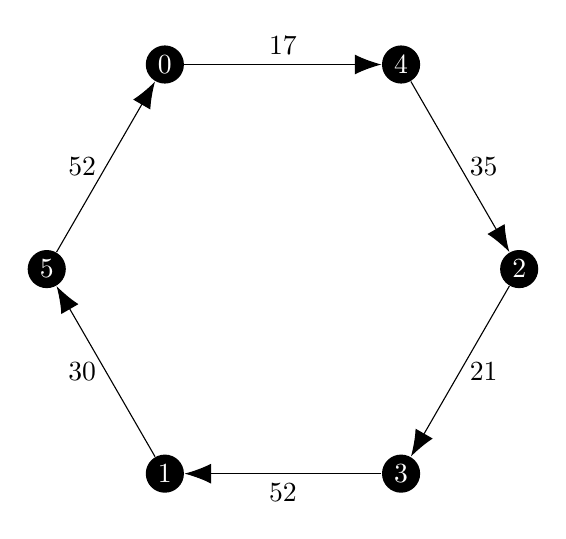
\begin{tikzpicture}
    \node[circle, inner sep=2pt, fill] (0) at (-1.5, 2.598) {\color{white} 0};
    \node[circle, inner sep=2pt, fill] (4) at (1.5, 2.598) {\color{white} 4};
    \node[circle, inner sep=2pt, fill] (2) at (3, 0) {\color{white} 2};
    \node[circle, inner sep=2pt, fill] (3) at (1.5, -2.598) {\color{white} 3};
    \node[circle, inner sep=2pt, fill] (1) at (-1.5, -2.598) {\color{white} 1};
    \node[circle, inner sep=2pt, fill] (5) at (-3, 0) {\color{white} 5};
    
    \draw[-{Latex[scale=2]}] (0) edge[above] node{17} (4);
    \draw[-{Latex[scale=2]}] (4) edge[right] node{35} (2);
    \draw[-{Latex[scale=2]}] (2) edge[right] node{21} (3);
    \draw[-{Latex[scale=2]}] (3) edge[below] node{52} (1);
    \draw[-{Latex[scale=2]}] (1) edge[left] node{30} (5);
    \draw[-{Latex[scale=2]}] (5) edge[left] node{52} (0);
\end{tikzpicture}
\hspace{1in}
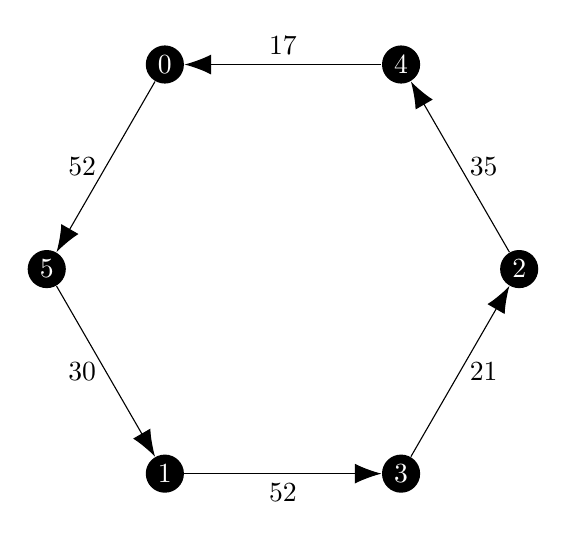
\begin{tikzpicture}
    \node[circle, inner sep=2pt, fill] (0) at (-1.5, 2.598) {\color{white} 0};
    \node[circle, inner sep=2pt, fill] (4) at (1.5, 2.598) {\color{white} 4};
    \node[circle, inner sep=2pt, fill] (2) at (3, 0) {\color{white} 2};
    \node[circle, inner sep=2pt, fill] (3) at (1.5, -2.598) {\color{white} 3};
    \node[circle, inner sep=2pt, fill] (1) at (-1.5, -2.598) {\color{white} 1};
    \node[circle, inner sep=2pt, fill] (5) at (-3, 0) {\color{white} 5};
    
    \draw[{Latex[scale=2]}-] (0) edge[above] node{17} (4);
    \draw[{Latex[scale=2]}-] (4) edge[right] node{35} (2);
    \draw[{Latex[scale=2]}-] (2) edge[right] node{21} (3);
    \draw[{Latex[scale=2]}-] (3) edge[below] node{52} (1);
    \draw[{Latex[scale=2]}-] (1) edge[left] node{30} (5);
    \draw[{Latex[scale=2]}-] (5) edge[left] node{52} (0);
\end{tikzpicture}
\end{document}